\section{Introduction partielle}
$ _{} $ $ _{} $ $ _{} $ $ _{} $ $ _{} $Dans ce chapitre, nous allons présenter brièvement le traitement automatique du langage naturel, ainsi que les techniques de traitement qui seront utiles pour la réalisation de l'objectif principal de ce travail. Nous allons donc y présenter une vue d'ensemble des architectures généralement utilisées, en nous focalisant essentiellement sur l'aspect intel\-li\-gence artificielle du \textit{NLP} (\textit{Natural Language Processing}).

Dans un premier temps, nous y présentons quelques techniques, souvent in\-con\-tour\-nables lorsqu'on veut réaliser une tâche de traitement du langage. Après cela, nous parcourons divers modèles qui nous permettrons d'aborder le modèle le plus adapté à la tâche de synthèse automatique des textes, qui est l'objectif de ce travail.
\section{Présentation et définitions}
$ _{} $ $ _{} $ $ _{} $ $ _{} $ $ _{} $Le NLP est une discipline rattachée à l'intelligence artificielle et ayant pour principal objectif, l'étude des possibilités du traitement du langage humain par des machines. La raison pour laquelle la discipline s'inscrit comme faisant partie du domaine d'intelligence artificielle est que le langage est considéré comme étant une aptitude centrale de l'intelligence humaine, étant donné que l'usage d'un langage si com\-ple\-xe est l'un des éléments distinctifs principaux entre humains et autres animaux.

Le NLP inclut l'ensemble d'algorithmes, des tâches et des problèmes prenant en entrée des textes produits par des humains, pour finalement ressortir des informations pertinentes à propos de ces derniers ou alors du texte modifié de façon appropriée selon l'objectif poursuivi. C'est ainsi que des tâches comme la traduction automatique, la génération automatique des textes ou aussi la synthèse automatique qui va nous intéresser dans ce travail, produisent directement du texte en sortie.

Mais, dans tous les cas, la sortie est soit immédiatement utilisable, soit alors elle est prise comme entrée d'un autre système dans la chaîne de traitement du texte.\\
On peut toutefois se demander la raison pour laquelle on parle de traitement automatique du "langage naturel" (quitte à se demander ce qui distinguerait un langage naturel des autres langages).

Pour établir clairement cette différence, il est nécessaire de donner une définition de ce qu'est un langage formel. Pour caricaturer, un langage formel est celui pour lequel il  existe un mécanisme fini, et explicite, permettant d'en faire une analyse, quand bien même il serait constitué d'un nombre infini de mots. Donc, c'est un ensemble de mots analysable par un automate (au sens mathématique du terme) \cite{carton2014langages}.

On peut donc comprendre directement que le mot "naturel" est ici utilisé pour faire une distinction avec \textit{les langages formels}. C'est donc dans ce sens que toutes les langues parlées peuvent être vues comme des langages naturels. Les langages formels ont une syntaxe précise et sont spécifiquement conçus pour des objectifs bien cernés (penser à tous les langages de programmation par exemple). Ils sont donc très précis tant au point de vu syntaxique que sémantique.

Concernant les langues humaines usuellement utilisées, on ne peut pas dire, sans être démenti, qu'elles sont dénuées d'imprécisions. Elles regorgent en générale une grande richesse, ce qui a pour conséquence d'introduire très souvent une grande ambiguïté. Pour s'en convaincre, il suffirait par exemple de considérer la phrase suivante :
\begin{center}
\textit{Je le vois avec mes jumelles.}
\end{center}
Très vite on remarque que cette phrase peut s'interpréter selon le contexte. On ne sait pas, en effet, si le sujet affirme voir quelqu'un avec ses jumelles d'observation, se promenant avec ses enfants jumelles, ou si le sujet voit quelque chose en utilisant ses jumelles en tant qu'instrument.\\
Ceci n'est qu'un exemple particulier pour illustrer cette dichotomie inhérente à l'emploi de la langue quelle qu'elle soit, mais cela suffit pour qu'on s'aperçoive que le problème est bel et bien réel.

Ce n'est d'ailleurs pas juste au niveau des interprétations qu'on peut identifier ce problème. Il s'observe même quand on considère les règles de grammaire. Certaines règles sont ainsi admises par certains linguistes mais rejetées ou trouvées superflues par d'autres \cite{jurafsky2014speech}.\\
C'est tout ce qui précède qui rend le langage humain à la fois riche et challengeant quand il s'agit de doter les machines de cette aptitude. D'où la raison d'être d'une discipline à part entière dédiée à la mise au point des règles de traitement du langage naturel, le NLP \cite{hagiwara2021real}.

\section{Nécessité de l'approche par deep learning}
$ _{} $ $ _{} $ $ _{} $ $ _{} $ $ _{} $Avant l'avènement du \textit{deep learning}, des techniques traditionnelles du NLP étaient u\-ti\-li\-sées pour des tâches comme la détection des spams, l'analyse des sentiments et le POS (Part Of Speech tagging). Ces approches utilisaient essentiellement des caractéristiques statistiques des séquences comme, la fréquence des mots et les co-occurences par exemple. Néanmoins, le principal désavantage de ces techniques était qu'elles ne parvenaient pas à capturer une grande partie de la complexité linguistique du langage humain, comme par exemple le contexte.

Ainsi, les développements, récents d'ailleurs, des réseaux de neurone et du \textit{deep learning} ont donné des nouveaux outils, pour approcher dans une large mesure les performances humaines en terme de traitement de langage. A notre avis, ces techniques sont les plus adaptées car, tout d'abord elles se rapprochent beaucoup plus des méthodes de traitement d'information par le cerveau humain, et ensuite, il serait autrement très couteux, voir impossible, d'élaborer des modèles capables d'embrasser toute la complexité du langage humain.

Le \textit{deep learning} pour le NLP est axé grosso-modo sur la représentation d'entités tex\-tu\-elles et le traitement élaboré sur ces représentations, de manière à en tirer des informations pertinentes ou à réaliser des transformations appropriées. Cette représentation constitue d'ailleurs un problème fondamental car c'est d'elle que dépend toute la chaîne de traitement des systèmes de NLP \cite{srivastava2021natural}.
\section{Quelques techniques courantes de traitement des textes}
$ _{} $ $ _{} $ $ _{} $ $ _{} $ $ _{} $Dans cette partie, nous allons présenter diverses techniques intervenant dans le trai\-te\-ment des données de langage naturel. Ces traitements seront présentés de manière à dégager un \textit{pattern} presque récurrent en terme de structure de traitement pour divers systèmes de NLP. Pour cela, nous allons d'abord présenter certaines manipulations réalisées sur les données en guise de pré-traitement. Puis, nous évoquerons deux techniques utiles aux tâches relevant du \textit{NLU (Natural Language Understanding)}.
\subsection{La tokenisation (\textit{tokenization})}
$ _{} $ $ _{} $ $ _{} $ $ _{} $ $ _{} $Manipuler des longues chaînes de caractères ne serait pas envisageable. Mais en informatique on est habitué à traiter des structures en terme de listes, de tableaux, de vecteurs,... Le tout étant représenté numériquement. C'est pour cela que l'opération consistant à réduire un corpus de texte en ses \textit{tokens} est centrale.\\
Dans notre contexte, la tokenisation est une opération qui consiste à décomposer un texte (une suite de phrases) en ses phrases constitutives ou une phrase en ses mots constitutifs. Cela est une première étape pour diminuer la difficulté inhérente au traitement des textes. En considérant la décomposition en mots, pour diminuer au maximum les difficultés de traitement et l'ambiguïté, on ajoute à la tokenisation d'autres traitements qui sont en général : \textbf{la désaccentuation}, \textbf{le passage aux minuscules}, \textbf{la suppression des \textit{stopwords}}, \textbf{la racinisation} et \textbf{la lemmatisation} appliqués aux tokens obtenus \cite{kulkarni2019natural}.\newpage
\subsection{Les \textit{stopwords} \cite{sarkar2019text}}
$ _{} $ $ _{} $ $ _{} $ $ _{} $ $ _{} $Les \textit{stopwords} sont, pour une langue donnée, des mots qui permettent de réaliser des phrases correctes mais qui n'apportent pas directement d'information significative sur l'ensemble (du point de vu traitement). Il s'agit par exemple en français de mots comme \textit{de, la, le,...} ce qui correspond, en gros, aux prépositions, aux articles, aux conjonctions,... Il faut néanmoins préciser qu'on peut très bien décider de ne pas supprimer certains \textit{stopwords}.
\subsection{La racinisation (\textit{stemming})}
$ _{} $ $ _{} $ $ _{} $ $ _{} $ $ _{} $La racinisation ou \textit{stemming} en anglais consiste à découper le token de manière à n'en conserver qu'une partie qui semble rendre mieux compte de ce dont dérive ledit token. Seulement, ceci est fait sans se fier à ce que le résultat obtenu en tant que racine fasse partie du dictionnaire de la langue considérée \cite{sarkar2019text,kulkarni2019natural}.\\
Cela permet juste de maximiser la probabilité de confondre des mots semblables qui sont présentés différemment dans diverses phrases. C'est à des fins de comparaison de phrases et de réduction d'ambiguïté. Pour illustration, on voudrait par exemple que si on retrouve les éléments "manger", "mange", "mangeable", "mangeons" dans un corpus, qu'ils soient transformés en un seul terme \underline{"mange"}. Cela se fait en découpant tous les mots qui ajoutent d'autres affixes au terme. C'est cela en bref le \textit{stemming} et, contrairement à ce que le nom suggère, il ne s'agit pas exactement de trouver la racine des mots (les mots dont ils dérivent). L'opération consiste essentiellement à réaliser un découpage des mots de manière à en supprimer les affixes.
\subsection{La lemmatisation (\textit{lemmatization})}
$ _{} $ $ _{} $ $ _{} $ $ _{} $ $ _{} $La lemmatisation quant à elle est une opération plus soignée mais plus coûteuse en terme d'implémentation \cite{sarkar2019text,kulkarni2019natural}. Elle réalise en fait ce qui n'est pas réalisé par le \textit{stemming} en ce sens que lemmatiser un token consiste à le transformer en sa racine, et cette dernière doit être présente dans le dictionnaire. Par exemple, pour un mot au pluriel, il s'agira de le remplacer par son singulier, un verbe conjugué, par son infinitif,... Pour illustration, la lemmatisation consisterait à transformer par exemple "va", "allions", "irons" et "allé" par \underline{"aller"} et "une", "des" par \underline{"un"}... Cette tâche est grandement facilitée par des techniques de deep learning.

L'obtention des tokens peut également conduire à des tâches plus élaborées comme \textbf{la détection des entités nommées} et \textbf{l'étiquetage morpho-syntaxique}. Il s'agit des tâches très importantes que nous devons nécessairement mentionner.
\subsection{Reconnaissance d'entités nommées (\textit{NER}) \cite{sarkar2019text}}
$ _{} $ $ _{} $ $ _{} $ $ _{} $ $ _{} $La détection des entités nommées (\textit{Named Entity Recognition} ou \textbf{NER}) consiste à repérer tout ce qui correspond à des noms de personnes, des noms d'organisations ou d'entreprises, des noms de lieux, des quantités, des distances, des valeurs, des dates ou tout autre élément qui constitue une nomination d'une entité existante précise dans un texte donné. Cette tâche est visiblement très importante dans la phase d'interprétation des données textuelles et il s'agit d'un simple problème de classification.
\subsection{L'étiquetage morpho-syntaxique (\textit{POS tagging})}
$ _{} $ $ _{} $ $ _{} $ $ _{} $ $ _{} $Le \textit{Part-Of-Speech tagging} est une tâche consistant en gros, à associer aux éléments des textes, des informations grammaticales. En général, il s'agit d'associer aux termes des textes, leur nature grammaticale. Cela consisterait à dire que tel élément est un nom, tel autre un verbe,...\cite{sarkar2019text,kulkarni2019natural}\\
Cette tâche n'est pas une fin en soi. En effet, c'est une première étape dans l'analyse structurelle des textes, permettant de déduire diverses dépendances du point de vu lin\-guis\-ti\-que. Elle est fortement facilitée par des approches basées sur le \textit{deep learning} comme c'est le cas aussi pour la reconnaissance d'entités nommées.

Nous allons passer sous silence certains autres concepts du NLP comme le \textbf{sacs de mots} et le \textbf{\textit{word embeddings}} dont nous parlerons dans la partie qui va suivre et qui présentera le résumé automatique, en tant que tâche du NLP.\newpage
\section{Approches du NLP}
$ _{} $ $ _{} $ $ _{} $ $ _{} $ $ _{} $Comme cela a été maintes fois mentionné, deux approches majeures sont d'usage pour traiter automatiquement les données de langage naturel. Il s'agit de l'approche numérique et de l'approche symbolique ou linguistique. Mais les deux approches sont dans la majorité des cas complétées par certaines heuristiques \cite{maaloul:tel-00756111}.\\
En ce qui nous concerne, l'approche sera essentiellement numérique avec un penchant prononcé pour les techniques du deep learning. D'ailleurs, concernant ces dernières techniques, les modèles de l'état de l'art les plus adaptés sont les \textbf{\textit{transformers}} et leur présentation exige une revue chronologique car en effet, pour y arriver, des modèles classiques basés sur des réseaux de neurones récurrents (\textit{RNN}) ont été utilisés car plus adaptés aux données séquentielles que sont les textes. Ensuite, le constat de leur mémoire limitée a fait à ce qu'on les modifie pour obtenir des unités à mémoire plus large dont les \textit{LSTM}(\textit{Long Short-Term Memory}) et les \textit{GRU}(\textit{Gated Recurrent Unit}). Furent ensuite introduits les mécanismes d'attention qui améliorèrent les techniques, aboutissant fi\-na\-le\-ment aux modèles dits \textit{\textbf{transformers}}, plus adaptés à des tâches de NLP élaborées.
\subsection{Les réseaux de neurones artificiels (\textit{ANN})}
$ _{} $ $ _{} $ $ _{} $ $ _{} $ $ _{} $Les réseaux de neurones artificiels (\textit{Artificial Neural Network} ou \textit{ANN}) sont un ensemble de neurones (artificiels) assemblés pour résoudre des tâches considérées comme requérant une certaine intelligence. Le neurone artificiel est un algorithme élaboré en s'inspirant du modèle théorique simplifié d'un neurone naturel. Il s'agit essentiellement d'une fonction d'agrégation ayant pour rôle de réaliser une somme pondérée des entrées qui lui sont présentées et d'une fonction d'activation qui formate la sortie de la fonction d'agrégation selon les valeurs attendues en sortie \cite{ANN}.\\
Les neurones sont généralement assemblés par couche comme présenté sur la figure qui suit :\newpage
\begin{center}
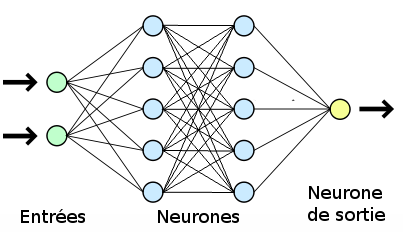
\includegraphics[width=13cm, height=7cm]{ANNsimple2.png}
\captionof{figure}{Réseau de neurones artificiel simple \cite{photANN}}
\end{center}
Ce qui vient d'être présenté est suffisant pour avoir une idée globale de ce qu'est réellement un réseau de neurones artificiel. Néanmoins, nous pousserons plus loin pour toucher le plus vite possible aux modèles qui nous intéressent dans ce travail.
\subsection{Les réseaux de neurones récurrents (\textit{RNN})}
$ _{} $ $ _{} $ $ _{} $ $ _{} $ $ _{} $Un \textit{RNN}(\textit{Recurrent Neural Network}) est un type de réseaux de neurones conçu en principe pour traiter les données séquentielles, comme les données textuelles,...\\
La principale différence structurelle entre les \textit{ANN simples} et les \textit{RNN} est l'existence des connexions de récurrence dans ces derniers. Il s'agit des boucles permettant la prise en compte des sorties passées dans le traitement final des données \cite{geron2020deep}.\\
Pour l'illustrer, rien de mieux qu'une image représentant la structure fonctionnelle des réseaux de neurones récurrents :\newpage
\begin{center}
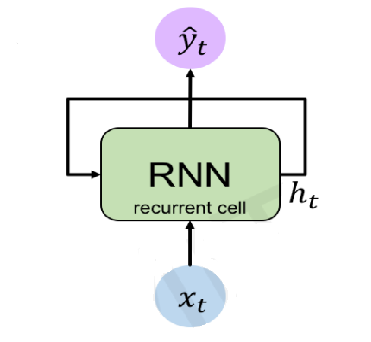
\includegraphics[height=4cm]{RnnsMIT2.png}
\captionof{figure}{Illustration de ce qu'est un RNN \cite{MITphot}}\label{IllustRNN}
\end{center}
Où $ x_{t} $, $ h_{t} $ et $ \hat{y}_{t} $ (à nommer juste $ y_{t} $) représentent respectivement les entrées, les états internes qui en résultent et les sorties (c'est-à-dire $ x $, $ h $ et $ y $ à chaque pas temporel $ t $).\\
Pour une meilleure compréhension, une présentation formelle serait plus commode :\\
Soient $ W_{x} $ la matrice des poids associée au vecteur d'entrée $ x $, $ W_{y} $ une matrice associée au vecteur de sortie $ y $ et $ W_{h} $ celle associée au vecteur représentant les états cachés du réseau, avec $ b_{h} $ et $ b_{y} $ respectivement les vecteurs des biais des neurones pour l'état caché et pour la sortie. On aura alors \cite{ganegedara2018natural} :
\begin{eqnarray}\label{eqRNN}
\begin{cases}
h_{t} &= f_{act}\left( W_{x}x_{t}+W_{h}h_{t-1}+ b_{h} \right)\\
y_{t} &= g_{act}\left( W_{y}h_{t} + b_{y} \right)
\end{cases}
\end{eqnarray}
On voit très bien que la sortie du système dépend non seulement de l'entrée, mais aussi de l'état du système ($ h $).\\
Les fonctions d'activation $ f_{act} $ et $ g_{act} $ qui sont mentionnées dans les équations \ref{eqRNN} représentent respectivement la \textit{tangente hyperbolique} $ tanh $ et la fonction dite $ softmax $ \cite{ganegedara2018natural}.

L'entraînement des réseaux de neurones récurrents se fait de la même façon que pour les réseaux de neurones simples (avec uniquement une différence due au fait que pour le \textit{RNN} on prend en compte le temps). On n'entrera pas dans le détail, vu que ce n'est pas exactement le sujet du travail mais, pour entamer la partie qui suit, il nous faut préciser que, comme pour les réseaux de neurones simples, l'entraînement exige d'appliquer une fonction de différentiation sur l'erreur produite par le système. Il s'agit de la fonction gradient. Mais, comme ici le gradient tient compte des grandeurs précédentes dans le temps, il y a un certain nombre de termes multiplicatifs qui peuvent amener le modèle à ne jamais converger ou au contraire, à la saturation. C'est le problème classique d'é\-va\-noui\-sse\-ment (disparition) des gradients ou d'explosion des gradients \cite{ganegedara2018natural}.\\
En réponse au problème de disparition des gradients, les cellules \textbf{\textit{LSTM}} (\textit{Long Short-Term Memory}) sont utilisées en lieu et place des cellules \textit{RNN} normales.
\subsubsection{Les cellules LSTM}
$ _{} $ $ _{} $ $ _{} $ $ _{} $ $ _{} $Les cellules \textit{LSTM} (pour \textit{Long Short-Term Memory}) sont utilisées en lieu et place des cellules \textit{RNN classiques} (dites \textit{vanilla}) pour permettre au réseau de traiter des séquences de plus en plus longues sans perte rapide d'information \cite{geron2020deep}. Pour cela, des éléments de contrôle de la mémoire de la cellule sont ajoutés. Pour illustrer nos propos, voici une image qui nous permettra de différencier une cellule RNN classique d'une cellule \textit{LSTM} :
\begin{center}
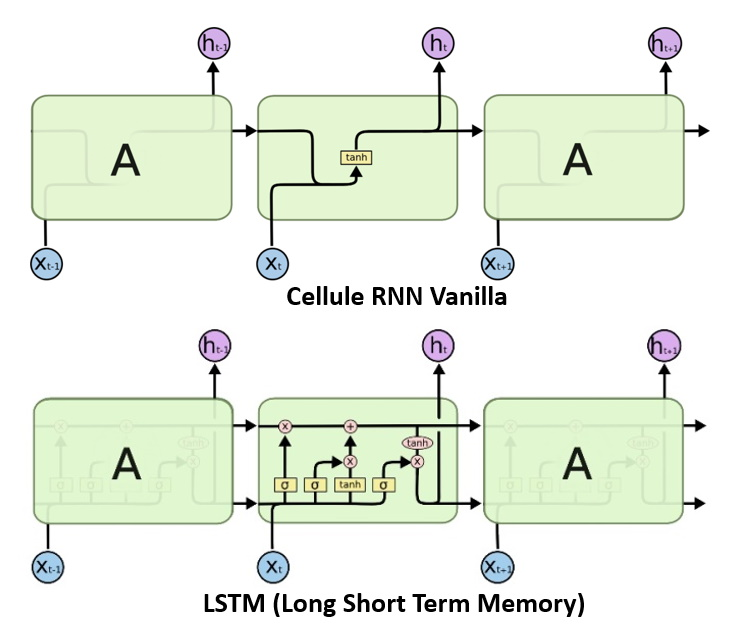
\includegraphics[height=10cm]{DiffRNN-LSTM.png}
\captionof{figure}{Comparaison entre cellules RNN classique et LSTM \cite{rnns}}
\end{center}
Présentée comme cela, la cellule \textit{LSTM} semble superflue mais si on présentait les équations associées à un réseau fait de ces cellules, on se rendra compte que c'est plutôt intuitif. Pour aborder les équations associées, considérons l'image suivante :\newpage
\begin{center}
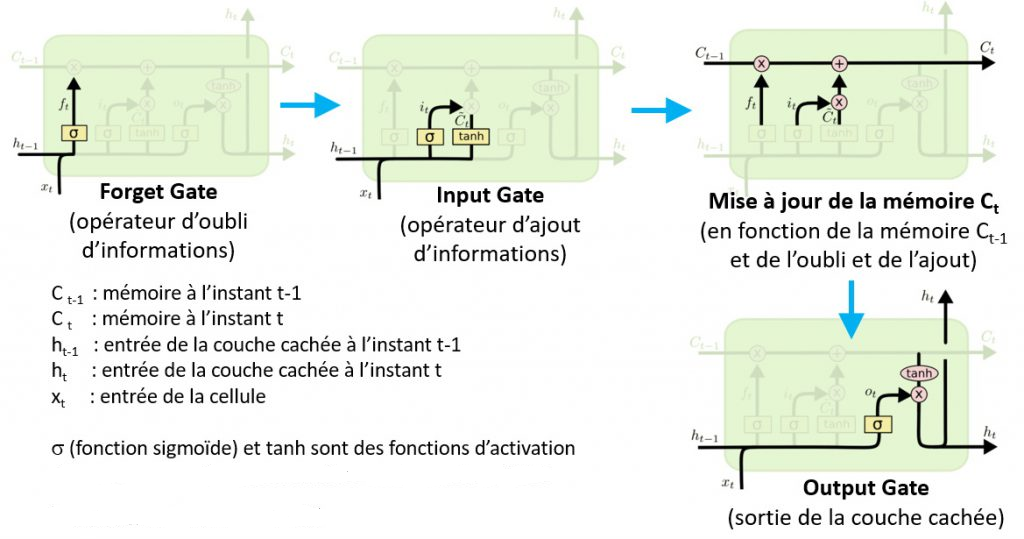
\includegraphics[width=16cm]{EqnLSTM.png}
\captionof{figure}{Vue fonctionnelle d'une cellule LSTM \cite{rnns}}
\end{center}
Une cellule \textit{LSTM} se comprend en la considérant comme constituée d'un ensemble de portes avec des fonctions bien particulières. Il s'agit d'une \textbf{porte d'entrée}, une \textbf{porte d'oubli} et une \textbf{porte de sortie}.\\
Il est évident que, pour chacune de ces portes que nous nommerons, à un instant $ t $ donné respectivement par $ I_{t} $, $ F_{t} $ et $ O_{t} $, le système doit apprendre ses paramètres en fonction de l'entrée et de l'état interne. Mais on doit aussi remarquer que, l'état est défini par deux paramètres au lieu d'un seul comme pour les RNN simples. Il s'agit, à un instant $ t $ donné, de $ h_{t} $ (considéré comme état à court terme) et de $ c_{t} $ (qui est un état à long terme mais dont le contenu est contrôlé, au vu de l'architecture de la cellule).\\
De ce que nous venons de dire, nous pouvons conclure que $ F_{t} $, $ I_{t} $ et $ O_{t} $ sont des fonctions de $ X_{t} $ et de $ h_{t-1} $ \textbf{aux poids près}. On sait aussi que, si on veut une mémoire à long terme contrôlée, la valeur finale de $ c_{t} $ doit être mise à jour en repérant ce qui doit être oublié parmi les éléments qui étaient précédemment dans la mémoire, pour y ajouter ensuite ce qui est sélectionné comme pertinent à l'entrée. Cela revient à utiliser $ F_{t} $ et $ I_{t} $ comme des portes de contrôle (ou de sélection). Et de cela on peut conclure que c'est plus intéressant d'avoir $ F_{t} $ et $ I_{t} $ qui prennent des valeurs entre $ 0 $ et $ 1 $ (pour modéliser la sélection) et $ c_{t} $ devra dépendre de ces deux éléments, avec aussi l'état précédent de la mémoire à long terme.\\
Il est aussi vraisemblable que, l'état à court terme doit provenir de la mémoire à long terme (ça correspondra à une sélection de ce qui doit être pris en compte directement dans la mémoire à long terme). Cet état $ h_{t} $ doit par conséquent dépendre de $ c_{t} $ (il faut néanmoins noter qu'une autre approche serait possible ici, mais celle-ci est déjà pertinente).\\
Finalement, on sait que la sortie finale doit nécessairement dépendre de l'état interne de la cellule. Il va ici s'agir de $ h_{t} $ vu que la cellule est développée par analogie avec le processus de mémorisation des systèmes naturels (mémoire à court terme correspondant à la mémoire de travail).

De ce qu'on vient de dire on peut tirer que, fondamentalement on doit avoir :
\begin{eqnarray}
\begin{cases}
F_{t} &= \mathcal{F}(X_{t},h_{t-1})\\
I_{t} &= \mathcal{G}(X_{t},h_{t-1})\\
O_{t} &= \mathcal{J}(X_{t},h_{t-1})\\
c_{t} &= \mathcal{K}(c_{t-1},X_{t},h_{t-1})\\
h_{t} &= \mathcal{L}(c_{t})\\
y_{t} &= \mathcal{M}(h_{t})
\end{cases}
\end{eqnarray}
Avec $ \mathcal{F}, \mathcal{G}, \mathcal{J}, \mathcal{K}, \mathcal{L}, \mathcal{M} $ des fonctions dépendant des coefficients considérés (poids et/ou éléments de sélection qui sont les diverses portes définies).\\
Une implémentation classique de ce raisonnement se présente comme suit \cite{geron2020deep,ganegedara2018natural} :
\begin{eqnarray}
\begin{cases}
F_{t} &= \sigma\left( W_{fx}X_{t}+W_{fh}h_{t-1}+b_{f} \right)\\
I_{t} &= \sigma\left( W_{ix}X_{t}+W_{fi}h_{t-1}+b_{i} \right)\\
O_{t} &= \sigma\left( W_{ox}X_{t}+W_{oh}h_{t-1}+b_{o} \right)\\
c_{t} &= F_{t}\circ c_{t-1} + I_{t}\circ \tanh\left( W_{cx}X_{t}+W_{ch}h_{t-1}+b_{c} \right)\\
h_{t} &= O_{t}\circ \tanh(c_{t})\\
y_{t} &= W_{yh}h_{t}+b_{y}
\end{cases}
\end{eqnarray}
Il faut remarquer qu'on a utilisé la fonction sigmoïde $ \sigma $ pour restreindre les valeurs des sélecteurs (portes) entre $ 0 $ et $ 1 $, puis on a utilisé le \textit{produit de Hadamard} (produit terme à terme des matrices) pour réaliser effectivement la sélection grâce aux portes, en diminuant les termes dont les valeurs correspondantes des portes sont proches de $ 0 $ et en essayant de conserver ceux dont les valeurs correspondantes des portes sont proches de $ 1 $.\\
Cette implémentation peut être modifiée, surtout en ce qui concerne les fonctions d'ac\-ti\-va\-tion utilisées ($ \sigma $ et $ \tanh $), et en particulier la fonction d'activation de finalisation $ \tanh $ ici, mais c'est l'une des plus optimales.

Le seul problème qui demeure est que le nombre de termes à apprendre est très grand. Cela a fait à ce qu'on puisse essayer de le diminuer en implémentant le \textit{\textbf{GRU}} (\textit{Gated Recurrent Unit}) poussant un peu plus loin l'abstraction des portes pour diminuer le nombre de paramètres.
\subsubsection{Les cellules GRU}
$ _{} $ $ _{} $ $ _{} $ $ _{} $ $ _{} $Les cellules \textit{GRU} (\textit{Gated Recurrent Unit}) sont une autre implémentation des cellules des réseaux de neurones récurrents comme les \textit{LSTM} à la différence près que, bien que partant de la même idée fondamentale évoquée précédemment, les \textit{GRU} apparaissent comme une simplification des \textit{LSTM}.\\
Elles possèdent néanmoins des performances comparables en ce qui concerne la prédiction des séries temporelles,... Les simplifications sont réalisées au niveau des états cachés et des portes. On conserve un seul état caché $ h $ (quitte à le contrôler à l'interne pour implémenter la mémorisation à long terme et à court terme). Et pour les portes, on fusionne les portes de sélection des entrées avec celle des éléments à oublier (donc les portes $ I $ et $ F $) pour former une porte dite de mise à jour (porte qui sera appelée \textit{update} ou $ U $). La porte de sélection des éléments de sortie quant à elle, est transformée en porte de réinitialisation.

Ces deux portes (de mise à jour et de réinitialisation) sont en fait implémentées de façon identique que celles des cellules \textit{LSTM}. La particularité des \textit{GRU} se situe prin\-ci\-pa\-le\-ment au niveau de la gestion de la mémoire (l'implémentation du processus de mémorisation) car, ayant supprimé la distinction long-terme/court-terme, il fallait bien trouver un mé\-ca\-ni\-sme devant permettre de bien gérer les deux aspects de la mémoire avec un seul état interne conservé.\\
C'est ainsi que, la porte de mise à jour (porte $ U $) est introduite dans le calcul de l'état $ h $ pour assurer la sélection du type de mise à jour à effectuer. Il s'agit de faire en sorte que, selon l'état interne et l'entrée, tout l'état interne précédent soit considéré  mais que certains éléments soient complètement modifiés, selon le besoin, et d'autres presque conservés.

Ainsi donc, $ h $ devient une combinaison d'éléments provenant de l'état interne précédent avec ceux provenant des nouveaux calculs effectués par la cellule (en fonction de l'entrée et de l'état interne précédent). Le comportement est alors le suivant :\\
Quand le vecteur de mise à jour a un terme proche de $ 1 $, cet état interne est presque conservé. Par conséquent, sa mise à jour est presque ignorée. Quand c'est plutôt $ 0 $, l'état interne précédent est presque ignorée et une mise à jour complète de cet état est effectuée. La formulation mathématique permet de mieux en saisir le fonctionnement \cite{geron2020deep,ganegedara2018natural} :
\begin{eqnarray}\label{EqnGRU}
\begin{cases}
U_{t} &= \sigma\left( W_{ux}X_{t}+W_{uh}h_{t-1}+b_{u} \right)\\
R_{t} &= \sigma\left( W_{rx}X_{t}+W_{ri}h_{t-1}+b_{r} \right)\\
h_{t} &= U_{t}\circ h_{t-1} + \left( 1-U_{t}\right)\circ \tanh\left( W_{hx}X_{t}+W_{hr}\left(R_{t} h_{t-1}\right) +b_{c} \right)\\
y_{t} &= W_{yh}h_{t}+b_{y}
\end{cases}
\end{eqnarray}
Et pour illustration, on peut considérer l'image suivante :
\begin{center}
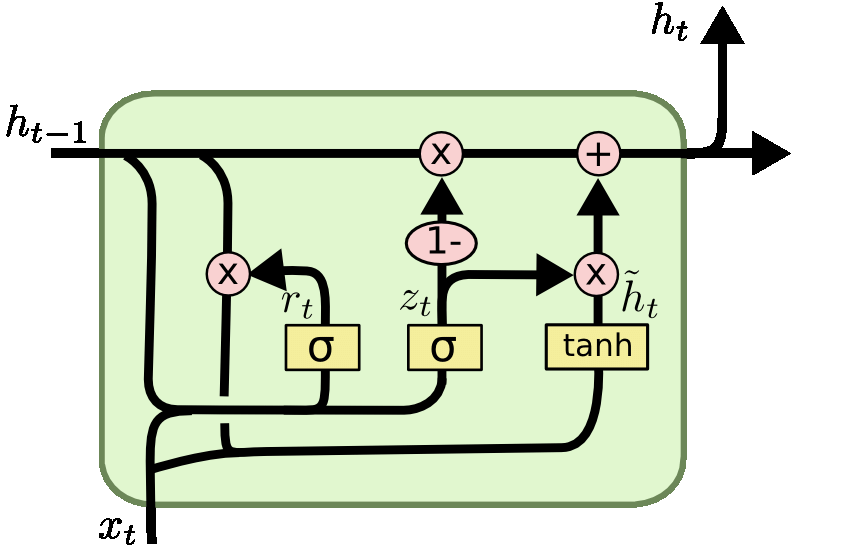
\includegraphics[scale=0.3]{Gated-Recurrent-Unit-GRU.png}
\captionof{figure}{Cellule GRU \cite{rnns}}\label{IllustGRU}
\end{center}
Il faut noter que sur cette image (figure \ref{IllustGRU}), l'implémentation de la mise à jour est l'inverse de celle que nous avons décrit par les équations \ref{EqnGRU}. C'est-à-dire que les termes $ U_{t} $ et $ \left( 1-U_{t}\right) $ sont permutés. Mais aussi, ici $ Z_{t} $ représente $ U_{t} $.\\

Ces modèles fonctionnent très bien et certaines implémentations permettent d'améliorer encore leurs performances. Ils sont néanmoins lents à entraîner, surtout à cause de l'aspect séquentiel. Parmi les techniques d'amélioration des performances, une peut être considérée car elle a un rapport direct avec notre travail. Il s'agit des \textbf{mécanismes d'attention} \cite{bahdanau2014neural}.\\
\subsection{Mécanismes d'attention}\label{AttentionEtseq2seq}
$ _{} $ $ _{} $ $ _{} $ $ _{} $ $ _{} $Les mécanismes d'attention sont en bref des techniques permettant de lutter contre la perte de mémoire qu'on constate par exemple dans les cellules récurrentes ci-haut décrites, en se focalisant sur des éléments les plus importants à chaque traitement. Le travail consiste donc à repérer, pour chaque entrée, les éléments sur lesquels se focaliser. C'est là qu'interviennent donc ces mécanismes.\\
L'une des implémentations les plus commodes est l'\textbf{attention globale} \cite{luong2015effective}.\\
Pour l'expliquer, nous allons considérer une architecture jusque là passée sous silence, mais qui permet aux modèles introduits là haut de s'utiliser efficacement pour les tâches courantes du \textit{NLP} en particulier. Il s'agit des modèles dits \textit{encodeur-décodeur}.\\
En effet, lorsqu'on a un modèle à séquence fonctionnel, les objectifs peuvent être multiples. On peut vouloir :
\begin{itemize}
\item[1°)] fournir une série d'éléments en entrée et ressortir une autre série (utile pour la prédiction de la valeur des actions par exemple,... );
\item[2°)] fournir un série en entrée mais faire ressortir un seul élément ou vecteur (utile pour la classification des textes, l'analyse des sentiments,...);
\item[3°)] fournir un vecteur plusieurs fois en entrée et produire une série (pour la génération des légendes pour des images par exemple,...);
\item[4°)] on peut aussi avoir un réseau série-vers-vecteur, appelé encodeur, suivi d'un réseau 
vecteur-vers-série, appelé décodeur (très utile pour la traduction et la synthèse au\-to\-ma\-ti\-que par exemple,...). Il s'agit du modèle \textbf{encodeur-décodeur}.
\end{itemize}
Une illustration par image sera suffisante :
\begin{center}
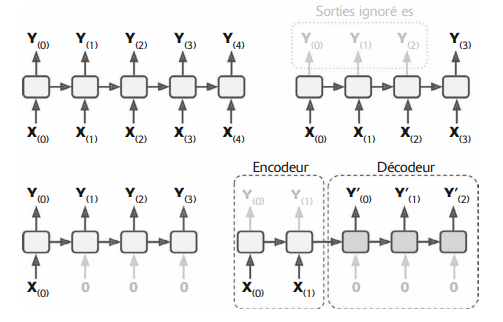
\includegraphics[scale=1]{IllustENC-DEC.PNG}
\captionof{figure}[Présentation des modèles encodeur-décodeur \cite{geron2020deep}]{Réseaux série-vers-série (en haut à gauche), série-vers-vecteur (en haut à droite), vecteur-vers-série (en bas à gauche) et encodeur-décodeur (en bas à droite) \cite{geron2020deep}}. \label{FigureSeq2Seq}
\end{center}
L'élément (le vecteur d'état) passé entre l'encodeur et le décodeur est dit \textbf{vecteur de contexte}. Il représente en quelques sortes un condensé des informations passés à l'entrée de l'encodeur. Toutefois, plus la séquence d'entrée est longue, plus le risque que la mémoire de certaines séquences puisse  s'étioler devient grand. Ainsi, si par exemple on est entrain de vouloir traduire une longue phrase, on peut finir par transmettre un vecteur de contexte qui a perdu toute information sur les premiers éléments de la séquence passée en entrée. C'est pour cela qu'au lieu de passer un vecteur de contexte général, les mé\-ca\-nis\-mes d'attention permettraient ici de ne se focaliser que sur certaines informations lors du traitement d'un élément particulier de la séquence (en ayant évidemment passé tous les états internes passés au décodeur). Pour le réaliser concrètement, le mécanisme d'attention global consiste à formater le vecteur de contexte en fonction des éléments de l'encodeur à prendre en compte lors du traitement par le décodeur.

Considérons que $ \Omega $, dont les termes sont représentés par $ w_{ij} $, est la matrice des poids d'attention normalisés par une fonction \textit{softmax} pour chaque ligne. Et que $ \Pi $, dont les termes sont représentés par $ \alpha_{ij} $, est la matrice des poids d'attention générée par le mé\-ca\-nis\-mes avant normalisation.Si les éléments $ c_{i} $ représentent à chaque fois le vecteur contexte final à l'étape $ i $ de décodage et les $ h_{j} $ sont les vecteurs d'état interne de l'encodeur, l'attention globale revient à réaliser la manipulation suivante, pour formater le vecteur de contexte à prendre en compte pour l'élément en cours de traitement \cite{luong2015effective} :
\begin{eqnarray}\label{EqnGlobAtt}
\begin{cases}
w_{ij} &= softmax(\alpha_{ij}) = \frac{e^{\alpha_{ij}}}{\sum_{k}e^{\alpha_{ik}}}\\
c_{i} &= \sum_{j}w_{ij}h_{j}
\end{cases}
\end{eqnarray}

La dernière relation du système \ref{EqnGlobAtt} revient à réaliser une somme pondérée des vecteurs d'état internes passés de l'encodeur, selon l'importance de chaque état pour le traitement en cours. De ces équations il faut aussi remarquer que la notation des sommations n'est pas rigoureuse. Cela est volontaire car c'est intuitif (on réalise des sommations sur tous les éléments).\\
Plusieurs techniques arrivant à réaliser l'attention existent. En général, comme on peut d'ailleurs le déduire des relations de l'attention globale, ces mé\-ca\-nis\-mes étaient utilisés dans le cadre des réseaux récurrents. Une question s'est toutefois naturellement posée : \textit{ne pourrait-on pas se passer des RNN pour mettre au point des réseaux complètement basés sur l'attention ?}. La réponse est oui, avec des ajustements adéquats pour résoudre les faiblesses des modèles classiques dans le traitement des données séquentielles. C'est cela qui a conduit aux modèles dits \textbf{\textit{transformers}} \cite{vaswani2017attention}.
\subsection{Les transformers}
Il s'agit des modèles dont l'architecture générique se présente comme suit :\newpage
\begin{center}
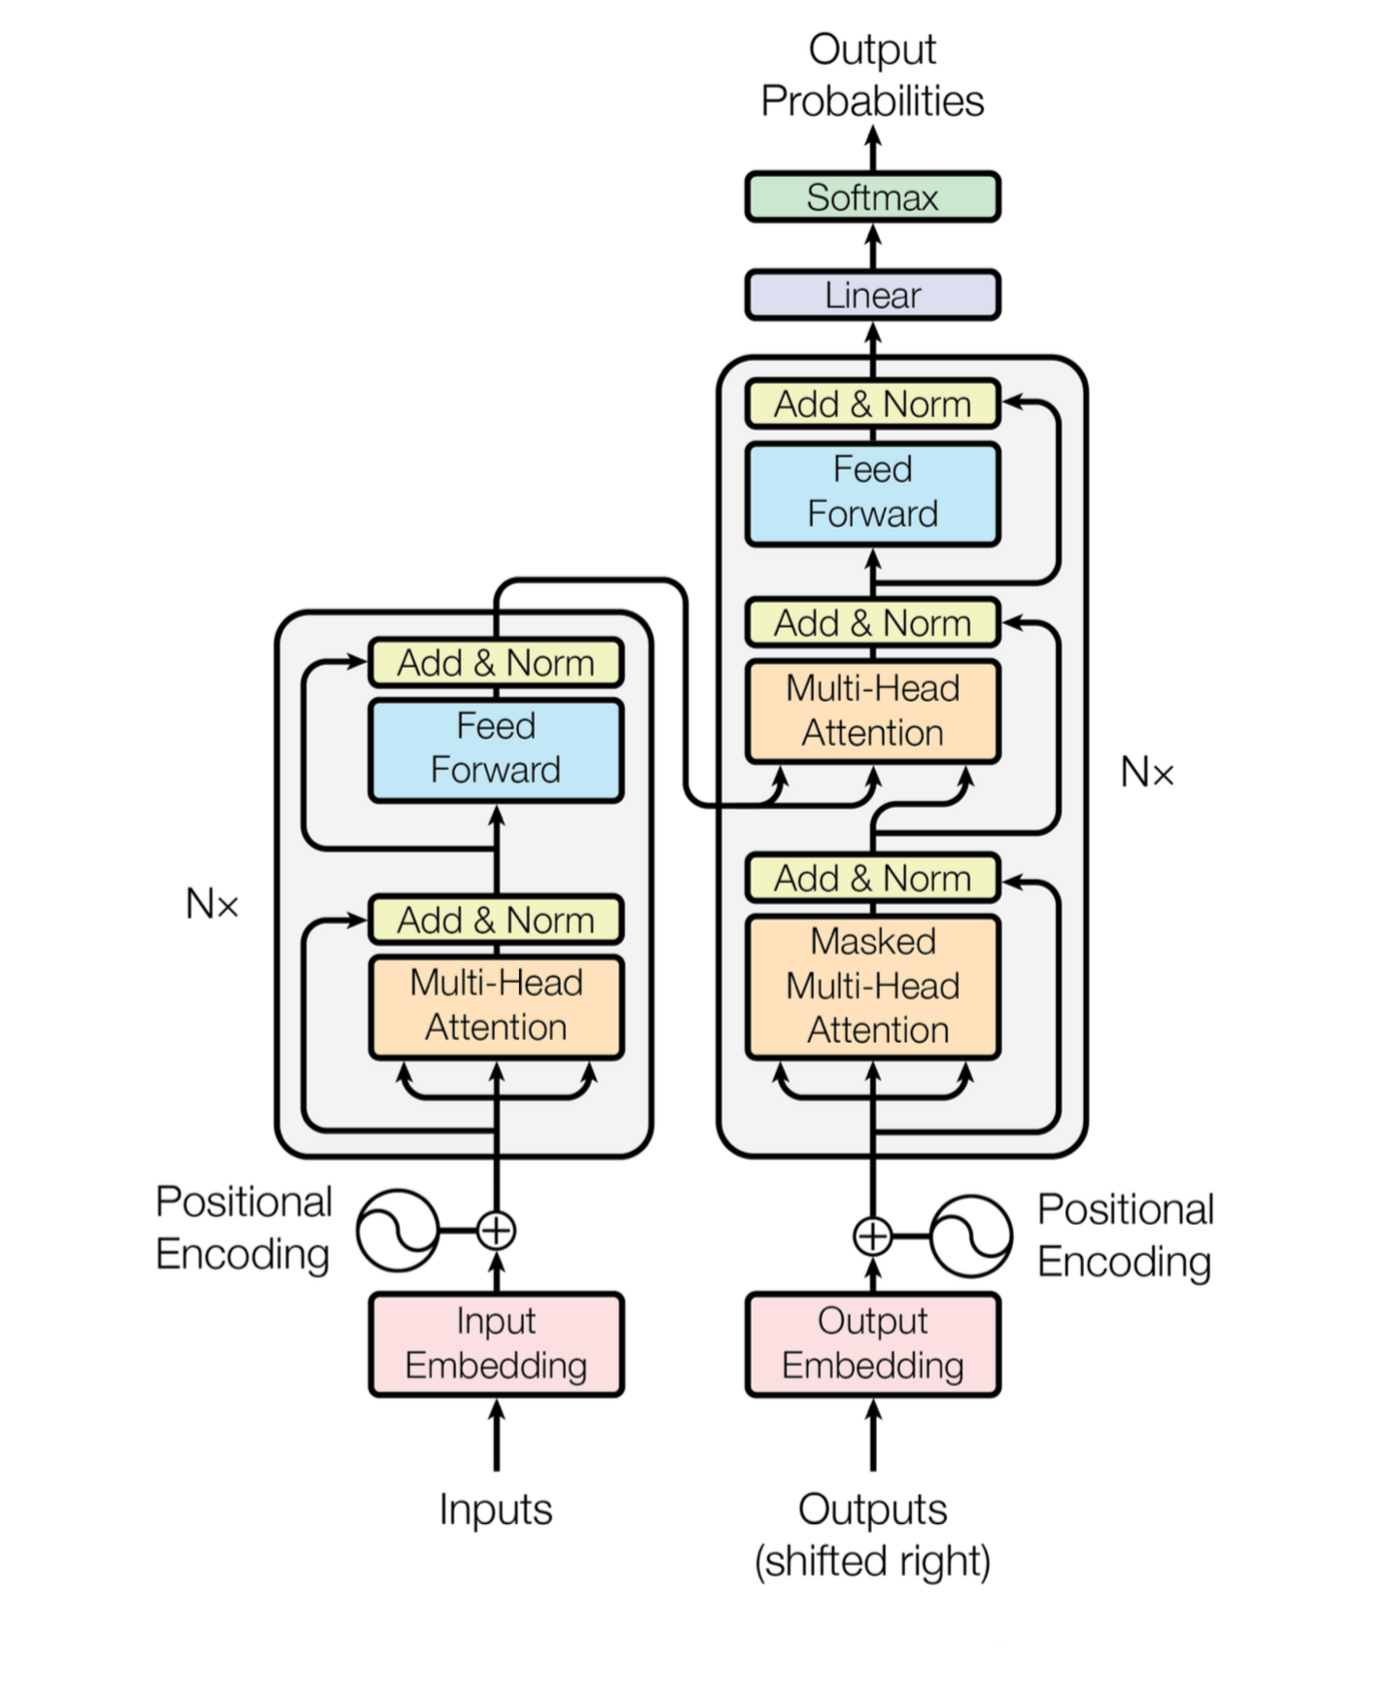
\includegraphics[scale=0.3]{TransformerVASWANI.PNG}
\captionof{figure}{Architecture générique des \textit{transformers} \cite{vaswani2017attention}}\label{ImgTransformerVASWANI}
\end{center}
Les \textit{transformers} sont des modèles du type \textit{encodeur-décodeur} comme on peut le constater sur la figure ci-dessus (bien que certaines implémentations n'en utilisent qu'une partie selon la tâche). Ils sont essentiellement basés sur les mécanismes d'attention, se passant de la récurrence \cite{geron2020deep,ganegedara2018natural}.\\
Nous donnerons une explication succincte de chacun des modules présents dans l'image \ref{ImgTransformerVASWANI}. En effet, présentons les modules selon l'ordre dans lequel les données traversent le modèle :
\begin{itemize}
\item[1°)] \textbf{Module d'embedding} : Nous savons que les données textuelles doivent être présentées au modèle sous forme numérique. Elles doivent donc être transformées avant de les passer aux parties suivantes. Néanmoins, vu que la représentation des entrées a un impact significatif sur les performances d'un modèle, cette représentation doit être bien choisie. Un choix intuitif, et qui s'avère être performant, est de tout faire pour que si deux termes ont des sens proches, ils aient aussi des représentations vectorielles proches. Cela est réalisé par différentes techniques que nous présenterons dans le chapitre suivant, mais c'est là le rôle de la couche d'enchâssement (\textit{embedding}).
\item[2°)] \textbf{L'encodage positionnel (\textit{positionnal encoding}}) : Ce module ajoute l'information sur la position relative de chacun des éléments placés en entrée par rapport aux autres. Cela pallie au problème de perte d'information sur la position des mots quand on utilise un réseau non séquentiel comme les réseaux récurrents. Donc, la position de chaque terme de la séquence placée en entrée est encodée dans un vecteur puis ajoutée à l'encodage global du terme. L'un des encodages les plus utilisés est celui basé sur les fonctions trigonométriques tel qu'introduit dans \cite{vaswani2017attention}.
\item[3°)] \textbf{Module d'auto-attention} :
La couche d'attention, présentée en première position dans la boîte de l'encodeur, est en fait une couche dite de \textit{self-attention} car elle opère sur la même séquence d'entrée. L'opération est réalisée pour permettre au modèle d'avoir une représentation de l'importance des termes dans la séquence d'entrée, les uns par rapport aux autres.\\
Pour illustration, considérons la phrase suivante : \textit{Walter est malade, il préfère se reposer}.\\
Dans cette phrase, l'un des constats qu'on peut faire est que, le nom "Walter" est beaucoup plus lié au pronom "il" qu'au verbe "préférer". C'est à l'établissement des tels liens dans les représentations que sert le module d'auto-attention ici présenté. Il est important que ce lien soit implicitement présent dans les représentations, pour que le traitement soit efficace comme on l'a mentionné lors de la présentation des mécanismes d'attention. Donc cette couche est en fait un prolongement de celle d'\textit{embedding}. Ici, le mécanisme d'attention utilisé est différent de celui qui a été présenté là-haut (attention globale). Il s'agit ici d'un mécanisme plutôt basé sur le produit scalaire mis à l'échelle (\textit{scaled dot-product}). En effet, très brièvement, l'idée du \textit{scaled dot-product attention} consiste à opérer une recherche des termes sur lesquels focaliser l'attention de la même façon qu'on réalise la recherche de la signification d'un mot dans un dictionnaire. Supposons qu'on veuille avoir la signification d'un mot dont on ne connaît pas l'orthographe exacte. Pour retrouver ce dernier dans un dictionnaire, il suffit de rechercher le mot qui ressemble le plus à l'orthographe que nous estimons être la plus vraisemblable. Mathématiquement, cette recherche de similitude correspond à un produit scalaire.\\
Similairement, le \textit{scaled dot-product} consiste à générer trois éléments qui sont \underline{la clé} ou \textit{key} $ k $, \underline{la valeur} ou \textit{value} $ v $ et \underline{la requête} ou \textit{query} $ q $. La \textit{requête} correspond au mot qu'on cherche (orthographié selon ce que nous pensons), la \textit{clé} correspond au mot présent dans le dictionnaire et la \textit{valeur} correspond à la signification associée. Si on supposait qu'il existe plusieurs termes du dictionnaire qui s'orthographient presque de la même façon que le mot qu'on cherche, on devra passer par une mesure de similarité avant de se décider sur le sens le plus probable. Cela correspond à réaliser le produit de tous les $ k $ par les $ q $ présents, puis à normaliser l'ensemble des résultats de manière à ce qu'ils représentent des mesures de probabilité, et finir par choisir le sens $ v $ le plus probable.\\
Pour aller plus vite, on implémente ce processus en considérant tous les $ k $, $ q $ et $ v $ au même moment de manière à réaliser le calcul une fois pour toutes. Cela revient à regrouper tous les $ k $, $ q $ et $ v $ dans des matrices $ K $, $ Q $ et $ V $. Ce qui donne la relation  qui définit l'attention par produit scalaire mis à l'échelle \cite{vaswani2017attention} :
\begin{eqnarray}\label{EqnScaledDotAtt}
Attention(Q,K,V) = softmax\left( \frac{Q\cdot K^{T}}{\sqrt{d_{k}}} \right)\cdot V
\end{eqnarray}
Dans cette relation, expression \ref{EqnScaledDotAtt}, le terme $ \sqrt{d_{k}} $ permet de mettre à l'échelle le résultat du produit scalaire de $ Q $ par $ K $, c'est-à-dire $ Q\cdot K^{T} $. Il faut noter que $ d_{k} $ est la dimension d'une clé, et que cette normalisation permet d'améliorer les performances du modèle mais elle n'est pas la seule envisageable.\\
Il est aussi important de remarquer que la couche d'attention utilise trois termes pour arriver à bout du problème. Ces trois termes sont obtenus par une transformation linéaire dont les poids sont appris à travers un réseau de neurones simple.\\
Il faut aussi noter que l'on utilise parallèlement plusieurs modules d'attention pour capture toutes les caractéristiques des séquences (on parle de \textit{multi-head attention}). Pour une plus ample illustration, voir la figure \ref{VueEclateeTrans}.
\item[4°)] \textbf{Le module \textit{feed-forward}} : Il s'agit en fait d'un réseau de neurones de propagation avant classique (réseau à couches ajoutées de façon séquentielle). Il permet de réaliser le traitement qui fait suite à l'attention.
\item[5°)] \textbf{Couche d'attention encodeur-décodeur} : Il s'agit de la couche qui reçoit les données en provenance de l'encodeur. Il s'agit ici d'une \textit{couche d'attention et non d'auto-attention} comme c'était le cas pour la première couche de l'encodeur. En effet, contrairement à la couche de \textit{self-attention}, pour laquelle tous les trois paramètres sont calculés à partir de la même séquence, la couche d'attention ici prend les clés $ K $ et valeurs $ V $ provenant de l'encodeur mais une requête $ Q $ provenant du décodeur.\\
Une autre couche \textit{feed-forward} suit celle-ci et a le même rôle que celle de l'encodeur.
\item[6°)] \textbf{Module d'attention masquée} : Il s'agit de la première couche du décodeur. C'est aussi un module de \textit{self-attention} auquel on ajoute le masquage. Ce module est dit masqué suite au fait que, comme le décodeur est un module de génération, on ne regarde que les termes précédemment générés, en masquant les termes qui seront probablement générés aux pas d'après. Cela est réalisé en rendant juste leurs probabilités nulles.
\item[7°)] \textbf{Module linéaire final} : Il s'agit d'un réseau de neurones classique pour réaliser la déduction finale, le tout étant passé à la fin à travers une opération \textbf{softmax} qui permet de transformer les résultats en probabilité d'éléments générés (cela permet de choisir le terme le plus vraisemblable à générer comme sortie).
\end{itemize}
Cette explication simplifiée se comprend mieux si on y joint la vue éclatée suivante :\newpage
\begin{center}
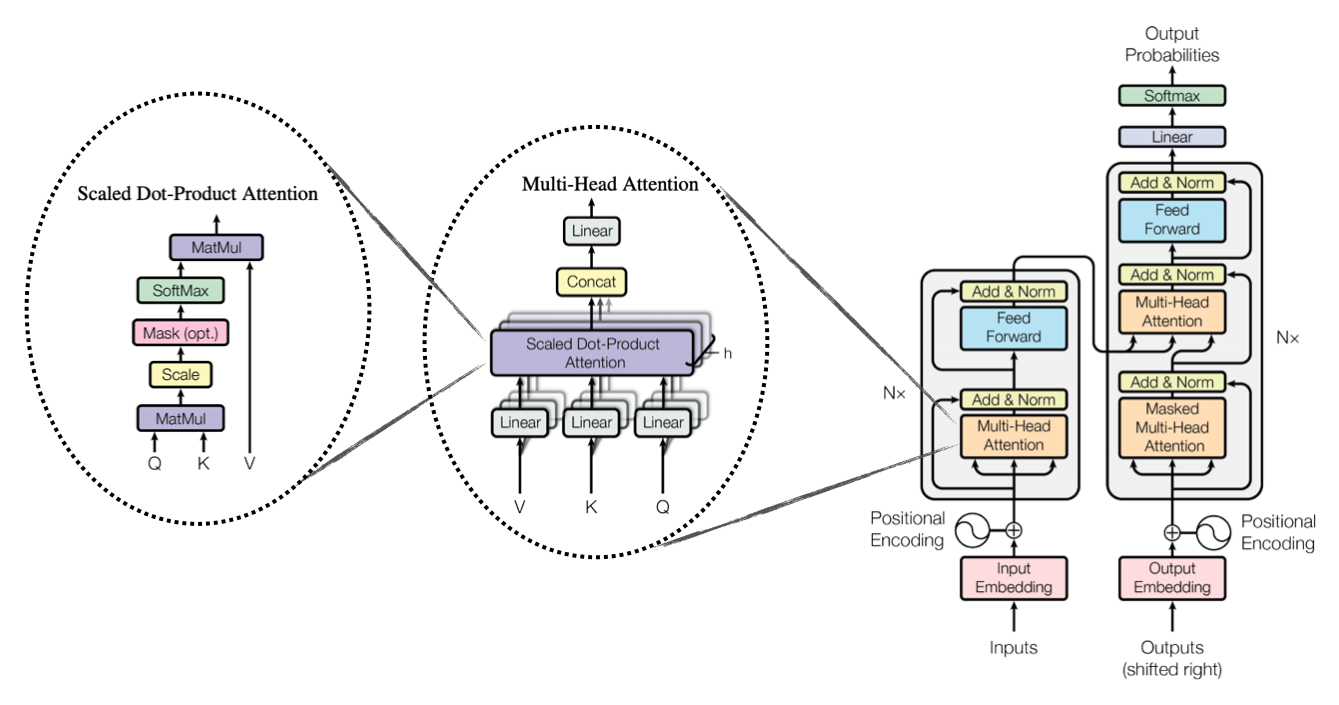
\includegraphics[width=16.5cm]{TransformerEclate2.PNG}
\captionof{figure}{Vue éclatée d'un transformer \cite{trans2020former}}\label{VueEclateeTrans}
\end{center}
Les \textit{transformers}, ici succinctement présentés, sont un modèle très adapté aux tâches de traitement automatique du langage naturel. C'est un modèle incontournable vu aussi que ses traitements peuvent être facilement parallélisés. Cela est rendu possible par le fait que l'architecture des \textit{transformers} est parallèle par essence. 
\section{Conclusion partielle}
$ _{} $ $ _{} $ $ _{} $ $ _{} $ $ _{} $Nous venons de réaliser une vue d'ensemble du domaine de traitement automatique du langage naturel, ainsi que diverses techniques couramment utilisées. Pour cela, nous avons tout d'abord justifié la préséance des modèles basés sur le \textit{deep learning} pour diverses tâches du NLP.\\
Ensuite, nous avons évoqué les technique de pré-traitement des textes, souvent in\-con\-tour\-na\-bles, comme la réduction des séquences en leurs tokens constitutifs, la suppression des mots fréquents mais n'apportant pas assez d'informations et la réduction des mots en leurs racines respectives. Nous y avons aussi joint quelques techniques utiles à la compréhension du langage humain comme le \textit{POS tagging} et la reconnaissance d'entités nommées. Ce qui précède nous a finalement conduit à présenter les modèles courants du NLP basés sur les RNNs et, nous avons terminé par la présentation de l'architecture \textit{transformer}, modèle que nous utiliserons pour ce travail (les précisions sur les modèles particuliers de \textit{transformer} à utiliser seront données au chapitre suivant).

Les transformers constituent un type de modèle qui s'avère être le plus adapté (pour le moment) au résumé automatique des textes et, dans le chapitre suivant, nous commencerons par présenter les diverses spécificités du résumé automatique comme tâche du NLP, pour finir par présenter l'architecture globale du système que nous comptons élaborer.